\section{DeepSmith}

DeepSmith\footnote{DeepSmith available at: https://chriscummins.cc/deepsmith}
is our open source framework for compiler fuzzing. Figure~\ref{fig:deeptune}
provides a high-level overview. The three key components of DeepSmith are: a
generative model for random programs, a test harness, and voting heuristics for
differential testing.

\begin{figure}[t!]
  \centering
  \begin{minipage}{.5\textwidth}
    \centering
    \vspace{-2em}
    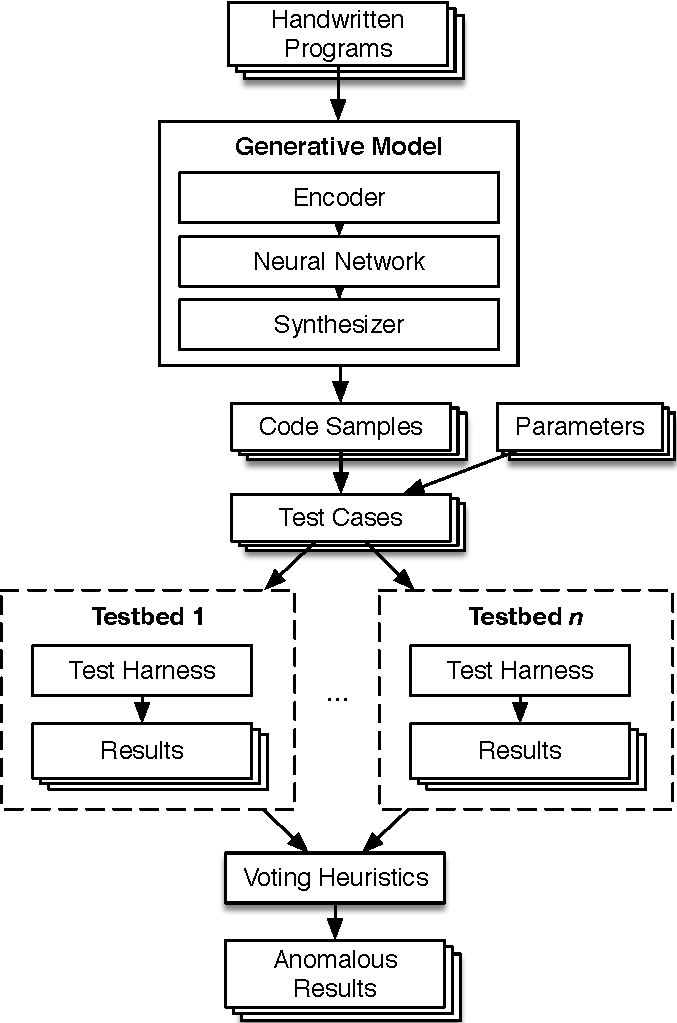
\includegraphics[width=.95\linewidth]{img/deepsmith}
    \captionof{figure}{DeepSmith system overview.}
    \vspace{-4em}
    \label{fig:deeptune}
  \end{minipage}%
  \begin{minipage}{.5\textwidth}
    \centering
    \vspace{-14em}
    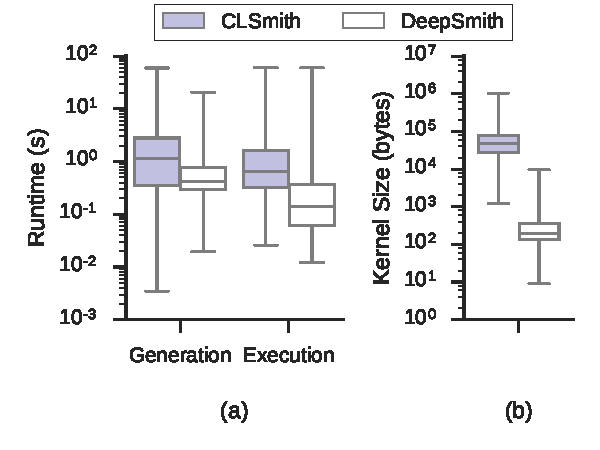
\includegraphics[width=\linewidth]{img/vs-clsmith}
    \vspace{-2.7em}
    \captionof{figure}{
      Comparison of runtimes (a) and test case sizes (b) of DeepSmith and
      CLSmith~\cite{Lidbury2015a}.
    }
    \label{fig:vs_clsmith}
  \end{minipage}\\*
  \begin{flushright}
    \begin{minipage}{.5\textwidth}
      \centering
      \vspace{-12em}
      \includegraphics[width=\linewidth]{img/clang-crashes}
      \vspace{-2em}
      \captionof{figure}{
        Crash rate of the Clang front-end of every LLVM release in the past 24
        months compiling 75k DeepSmith kernels.
      }
      \label{fig:clangs}
    \end{minipage}
  \end{flushright}
\end{figure}

\vspace{-.5em}
\paragraph{Generative Model} We treat the generation of compiler testing inputs
as an unsupervised machine learning task, employing state-of-the-art deep
learning techniques to build models for how humans write programs. To generate
inputs for testing OpenCL compilers, we train a Recurrent Neural Network on a
corpus of handwritten code, assembled by mining 10k OpenCL kernels from open
source repositories on GitHub~\cite{Cummins2017a}. We used an
\emph{oracle compiler} (LLVM 3.9) to statically check the source files,
discarding files that are not well-formed. This corpus, exceeding one million
lines of code, is encoded using a hybrid keyword and character level
tokenizer~\cite{Cummins2017b}. Training the model on the OpenCL corpus took 12
hours using a single NVIDIA Tesla P40. We provided the model with no prior
knowledge of the structure or syntax of a programming language. The trained
network is sampled to generate new programs. To generate a new program, the
model is seeded with the start of a program, and sampled token-by-token. A
``bracket depth'' counter is incremented or decremented upon production of
\texttt{\{} or \texttt{\}} tokens respectively, so that the end of the program
can be detected and sampling halted.

\vspace{-1em}
\paragraph{Test Harness} We developed a harness to execute generated OpenCL
programs. The harness accepts an arbitrary OpenCL program, generates input data
for it, and executes the program on an OpenCL device. Unlike the generative
model, this test harness is language-specific and the design stems from domain
knowledge. Still, it is a relatively simple procedure, consisting of a few
hundred lines of Python.

\vspace{-1em}
\paragraph{Voting Heuristics} We employ established Differential Testing
methodologies to expose compiler defects. We look for test cases where there is
a majority outcome -- i.e. for which some fraction of the testbeds behave the
same -- but some testbed deviates. We use the presence of the majority
increasing the likelihood that there is a `correct' behavior for the test case.
A series of heuristics detect common causes of undefined behavior and remove
false positives.
